\section{Clustering}

% Principalmente, el proceso de desagregacion de preguntas del conjunto de datos  VizWiz-VQA, fue llevado a cabo utilizando como columna vertebral, el clásico algoritmo de aprendizaje no supervisado llamado `KMeans' de la libreria sklearn. Este, al no requerir supervisión ni etiquetado previo, es muy útil para explorar conjuntos con estructuras y distribuciones no  conocidas. Mediante la determinación iterativa de centroides, este método permite agrupar datos de características similares según la distancia a la que se encuentren del centroide mas cercano.
Mainly, the question disaggregation process of the VizWiz-VQA dataset was carried out using as a backbone, the classic unsupervised learning algorithm called \emph{KMeans} from the sklearn library\footnote{\url{https://scikit-learn.org/stable/index.html}}. This, as it does not require supervision or prior labeling, is very useful for exploring datasets with unknown structures and distributions. Through the iterative determination of centroids, this method allows data with similar characteristics to be grouped according to their distance from the closest centroid.

% Como en cualquier otro modelo de aprendizaje automático, KMeans, también requiere que sus datos de entrada sean representaciones numéricas. Es por ello, que se probaron varias estrategias para mapear secuencias de palabras (preguntas, preguntas+respuestas, etc), a sus respectivos vectores de características.
Like any other machine learning model, KMeans also requires that its input data be numeric representations. For this reason, various strategies were tested to map sequences of words (questions, questions + answers, etc.) to their respective feature vectors.

\subsection{Data preprocessing}
% Como primera fase, se procedió a realizar un proceso de curado del conjunto de datos VizWiz-VQA. Dado a que todos los análisis estuvieron dirigidos a preguntas y respuestas; y el grupo de testeo no contiene respuestas asociadas, sólo se utilizaron datos de los conjuntos de entrenamiento y validación.
As a first phase, a curing process of the VizWiz-VQA dataset was carried out. As all the analyzes were carried out on the questions and the answers, only the data corresponding to the training and validation sets were used, since the test set does not contain associated answers.

% El primer paso, fue realizar la normalización de cada una de las preguntas. Mediante la utilizando de la libreria `contractions', se expandieron las contracciones, filtraron caracteres no alfabéticos y se transformaron a minúsculas. Luego, posterior a la supresión de los espacios en blanco iniciales y finales, con la ayuda de la librería de NLP spacy, se filtraron preguntas con más de una sentencia, y eliminaron duplicadas. Recordar que, al ser un dataset de naturaleza conversacional, muchas preguntas son de gran longitud, y contienen información irrelevante que potencialmente podrían introducir ruido en el proceso de clusterización.
The first step was to normalize each of the questions. Using the \emph{contractions}\footnote{\url{https://pypi.org/project/contractions/}} library, the contractions were expanded, non-alphabetic characters filtered out, and converted to lowercase. Then, after deleting the leading and trailing blanks, with the help of the NLP \emph{spaCy}\footnote{\url{https://spacy.io/}} library, the questions were filtered with more than one sentence. Later, the duplicate questions were also eliminated. 
Remember that as this is a conversational dataset, many questions are very long and contain irrelevant information that could introduce noise into the clustering process.

% El resultado de estos procedimientos, culminó con 9003 pares de preguntas/respuestas únicas, de un total inicial de
% 24842 pares. En el proceso, las 10 respuestas asociadas a cada pregunta fueron re-ordenadas de manera decreciente en una lista de tuplas de la forma (respuesta, numero de coincidencias). La Figura (\ref{fig:frec_word_qs}), muestra la distribución final de las 50 palabras más frecuentes contenidas en las 9003 preguntas. Por otro lado, en la Figura(\ref{fig:wc_ans}), se visualizan las 100 respuestas más frecuentes, considerando (no considerando) las destacada `unsuitable` y `unanswerable' respectivamente.
The result of these procedures culminated in 9003 unique pairs of questions and answers, out of an initial total of 24842 pairs. In the process, the 10 responses associated with each question were re-ordered in descending order in a list of tuples of the form (response, number of matches). Figure (\ref{fig:frec_word_qs}), shows the final distribution of the 50 most frequent words contained in the 9003 questions. On the other hand, in Figure (\ref{fig:wc_ans}), the 100 most frequent answers are displayed as cloud word style, considering (not considering) the two most frequent answers `unsuitable' and `unanswerable' respectively.

\begin{figure*}[ht!]
    \centering
    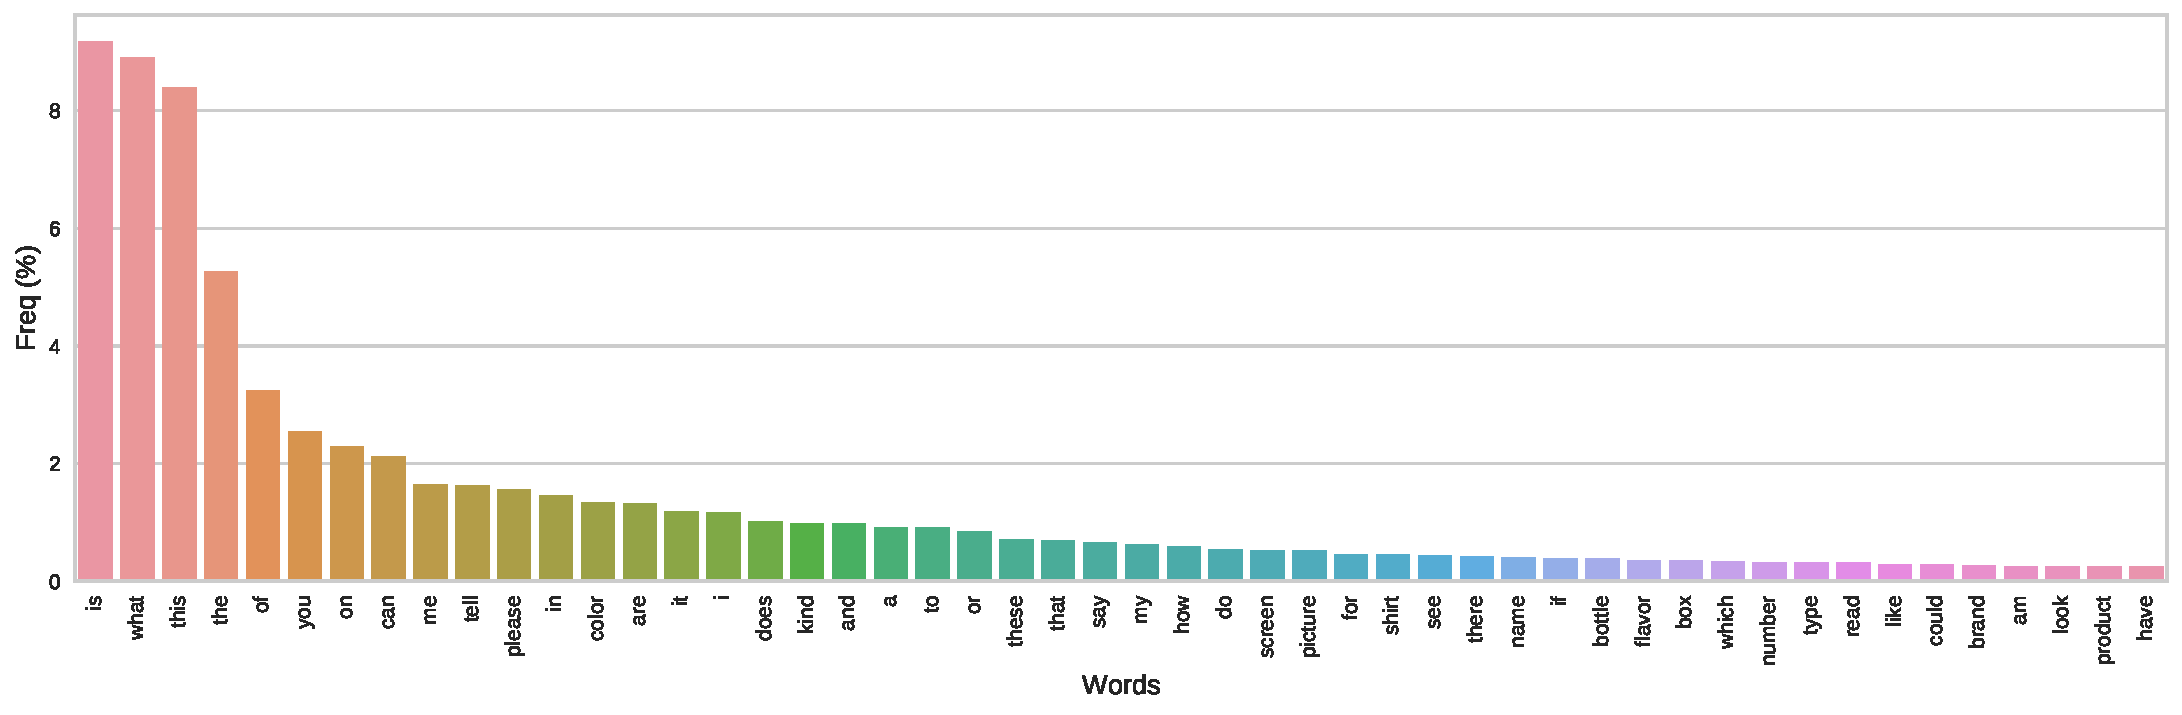
\includegraphics[width=\linewidth]{images/pre/fd_top50_qs_words.pdf}
 \caption{The 50 most frequent words in VizWiz-VQA questions dataset.}
\label{fig:frec_word_qs}
\end{figure*}


\begin{figure}[ht!]
    \centering
    \begin{minipage}[c]{0.49\linewidth}
        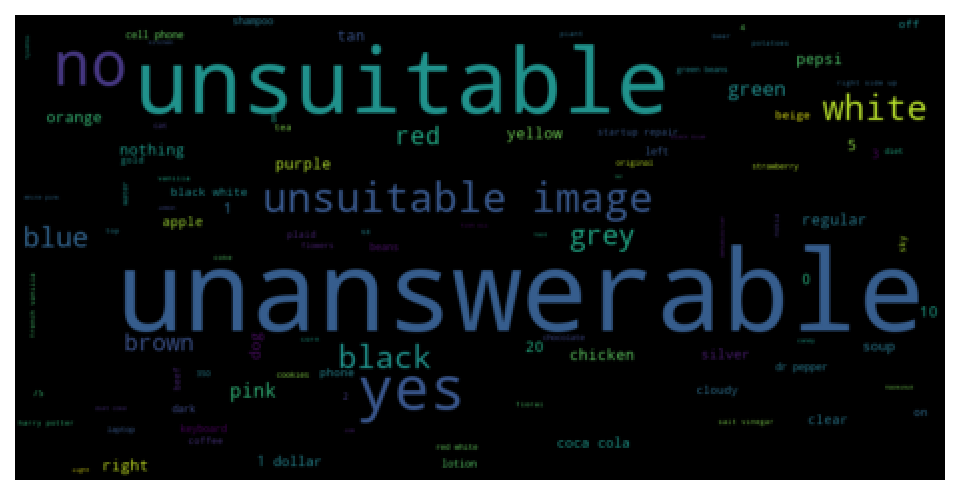
\includegraphics[width=\textwidth]{images/pre/wc_top100_best_ans.pdf}
    \end{minipage}
    %
    \begin{minipage}[c]{0.49\linewidth}
        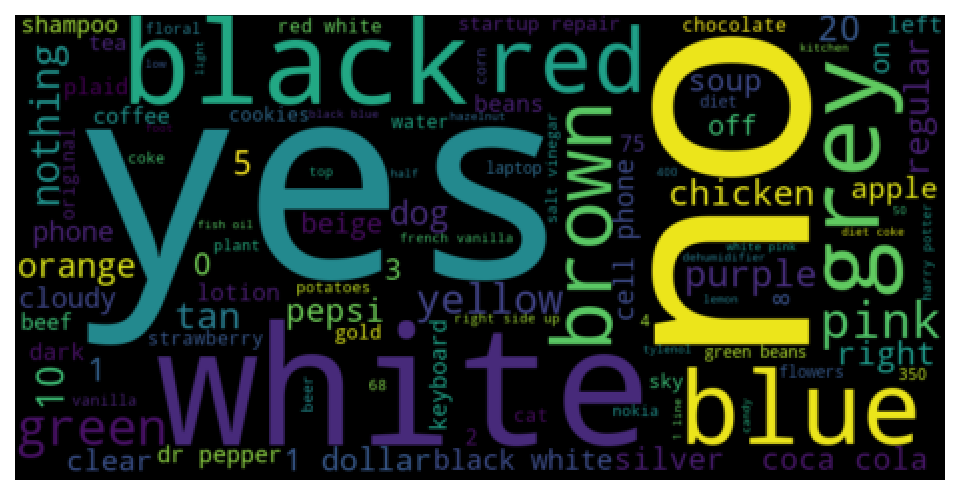
\includegraphics[width=\textwidth]{images/pre/wc_top100_best_ans_red.pdf}
    \end{minipage}
    \caption{The 100 most frequents answers in the VizWiz-VQA dataset. (Left): With 'unsuitable' and `unanswerable' answers. (Right): Without 'unsuitable' and `unanswerable' answers)}
    \label{fig:wc_ans}
\end{figure}

\subsection{Data representations}
% Para la representación de los datos, se utilizaron dos diferentes tipos de embedding: I) embedding basados en matrices de ocurrencia + reducción de dimensionalidad; y II) embedding obtenidos de modelos neuronales pre-entrenados.
For the representation of the data, two different types of embedding were used: I) embedding based on occurrence matrices + dimensionality reduction; and II) embedding obtained from pre-trained neural models.

% Para el primer tipo (I), se testearon distintas combinaciones de concatenaciones de datos de entrada. Mediante el uso de la librería `spacy', se probaron: ``lista de lemas de preguntas'', ``listas de lemas de preguntas + lista de lemas de mejor respuesta'', ``lista de lemas de preguntas + lista de lemas de todas las respuestas''; y de igual  forma con combinaciones de palabras sin lematizar y PoS (Part of speech) de las preguntas. Cabe aclarar que en las concatenaciones resultantes, para poder diferenciar los lemas pertenecientes a las preguntas de los pertenecientes a las respuestas, se añadieron tokens especiales \emph{CLS} y \emph{SEP}, ubicados al inicio y final de cada lista.
For type (I), different combinations of input data concatenations were tested. Using the \emph{spaCy} library, the following were tested: `question lemma list', `question lemma lists + best answer lemma list', `question lemma list + all answer lemma list'; in the same way with combinations of words without stemming and PoS (Part of Speech) of the questions. It should be noted that in the resulting concatenations, in order to differentiate the lemmas belonging to the questions from those belonging to the answers, the special tokens \textbf{CLS} and \textbf{SEP} were added, located at the beginning and end of each list.

% La construcción de las matrices de ocurrencia fueron realizadas utilizando diferentes rangos de n-gramas, desde (1-grama,..,3-grama) hasta un máximo de (1-grama,...,10-gramas). Posterior a esto, se realizó la reducción de dimensionalidad mediante un humbral de varianza. La misma, se implementó a través del método VarianceThreshold de `sklearn', entregando vectores de dimensiones que oscilaron entre 90 y 120.
The construction of the occurrence matrices were performed using different ranges of n-grams, from (1-gram,..,3-gram) to a maximum of (1-gram,...,10-grams). After this, the dimensionality reduction was performed using a variance threshold. It was implemented through the \emph{varianceThreshold} method of the \emph{sklearn} library, providing vectors with dimensions that ranged from 90 to 120.

% Para el segundo tipo de embedding (II), se probaron codificaciones usando modelos pre-entrenados a nivel de palabras, mediante \textbf{fastText}, y a nivel de sentencias, mediante \textbf{doc2Vec}; ambos pertenecientes a la libreria `gensim'. En el caso particular de `fastText', se emplearon dos estrategias en para la obtención del embedding resultante. Por un lado se uso una sumatoria (elemento a elemento), y por el otro una multiplicación, de cada uno de los embedding individuales codificados.
For the type of embedding (II), encodings were tested using pre-trained models at the word level, using \emph{fastText}, and at the sentence level, using \emph{doc2Vec}; both from the \emph{gensim}\footnote{\url{https://pypi.org/project/gensim/}} library. For the particular case of the \emph{fastText} model, two strategies were used to obtain the resulting embedding: summation of individual embedding on the one hand, and multiplication of individual embedding on the other.

\subsection{First approach}
\label{subsec:first_approach}
% Como primera aproximación al problema, se realizaron una sucesión de ejecuciones del algoritmo KMeans, utilizando diferentes rangos de valores de k (k=número de clusteres deseados). La evaluación de resultados fue efectuada de manera visual y cualitativa, ayudándose de la generación de gráficas de Silohuette que guiaron el proceso de selección de los valores k más óptimos. A rasgos generales, en este primer contacto, se busco reducir el conjunto de variables y configuraciones que arrojaran mejores agrupaciones, y conocer el trasfondo del comportamiento de los resultados.
As a first approximation to the problem, a succession of executions of the KMeans algorithm were carried out, using different ranges of k values, where $k=number\_of\_desired\_clusters$. The evaluation of the results was carried out visually and qualitatively, with the help of the generation of Silohuette graphs that guided the selection process of the most optimal k values. In general terms, in this first contact, we sought to reduce the set of variables and configurations that would yield better groupings, and to know the background of the behavior of the results.

% De tales pruebas, se observó que muchas preguntas del estilo: \emph{`please, can you tell me what is in this box?'} y \emph{`what is in this can?'}, eran ubicadas en clusteres diferentes a pesar de poseer semánticas similares. Luego de realizar una revisión detallada del conjunto completo, se identificó que ciertas oraciones de naturaleza conversacional, que precedían a las preguntas, eran las responsables de confundir al algoritmo de clusterización; una lista completa de todas las secuencias identificadas puede ser encontrada en Anexo (). Tal hallazgo, forzó a un nuevo re-procesamiento de datos, y re-generación de listas de `lemas', `PoS' y `tokens' utilizados en la generación de cada embedding. Ahora, cada vez que una sentencia de estas características era identificada como sub-secuencia de una pregunta, sus tokens no eran añadidos a las listas.
% Otro aspecto importante observado, fue que combinaciones de entrada basadas en lista de PoS y palabras sin lematizar, entregaban resultados muchos menos precisos que al usar diferentes combinaciones de listas de lemas.
From such tests, it was observed that many questions like: \ emph {`please can you tell me what's in this box? '} And \ emph {`what's in this can?'}, They were placed in different clusters, despite having similar semantics. After conducting a detailed review of the complete set, it was identified that certain conversational sentences located at the beginning of the questions, were responsible for confusing the grouping algorithm. A complete list of all identified sequences can be found in the Annex (\ref{app:conversational_seq}). This finding forced a new data re-processing, and re-generation of lists of `lemmas', `PoS' and `tokens' used in the generation of each embedding. Now, every time a statement of these characteristics was identified as a sub-sequence of a question, its tokens were not added to the lists.
Another important aspect observed was that input combinations based on Part of Speech lists and non-stemmed words, gave much less accurate results than when using different combinations of lemmas lists.

\subsection{Selection of the best strategy}
\label{subsec:best_strategy}
% Con toda la información obtenida de la primera aproximación, y teniendo en cuenta el objetivo principal de desagregar las categorías mayoritarias de VizWiz-VQA, mediante los grupos de preguntas retornadas por el algoritmo de clusterización; en esta segunda etapa, se incorporaron métodos de testeo mas sistemáticos para poder cuantificar la calidad de los resultados.
With all the information obtained from the first approximation (\ref{subsec:first_approach}), and given the main objective of disaggregating the majority categories of VizWiz-VQA through the groups of questions returned by the clustering algorithm; In this second stage, more systematic testing methods were incorporated in order to quantify the quality of the results.

% Uno de ellos, fue el conocido método de Elbow (o método del codo). Este es un a heurística que se usa para determinar el número de clusters en un conjunto de datos. Este método gráfica la variabilidad como función del número de clusters, y selecciona el `codo' de la curva  como el número de clusters a utilizar. A pesar de que se testearon amplios rangos de valores (entre 3 y 20), todas las curvas obtenidas tenian un comportamiento bastante lineal, por lo que sus resultados no fueron de mucha utilidad.
One of them was the well-known \emph{Elbow} method. This is a heuristic used to determine the number of clusters in a data set. This method graphs the variability as a function of the number of clusters, and selects the `elbow' of the curve as the number of clusters to use. Although wide ranges of values were tested (between 3 and 20), all the curves obtained had a fairly linear behavior, so their results were not very useful.

% Como segundo método de testeo, se confeccionó un conjunto de datos de pruebas, formado de N tuplas de preguntas aleatorias, seleccionadas de entre las 9003 del conjunto de datos filtrados. Se etiqueto cada par con `Si' (`No'), acorde a si las preguntas deberían (o no) pertenecer al mismo cluster.
As a second method, a test dataset was made, made up of N tuples of random questions, selected from among the 9003 of the filtered data set. Each pair was labeled with Yes/No, according to whether the questions should/or not, belong to the same cluster.
% En total fueron anotados 230 pares, y se calcularon los porcentajes de acierto, tanto para aquellos en que la tupla de preguntas caían en un mismo cluster, coincidiendo con la anotación manual, y viceversa para los que no lo hacían.
% A pesar de que esta última estrategia arrojó datos estadísticos muy útiles para la selección de la mejor estrategia, se necesitó de una supervisión humana adicional para  determinar la validez y consistencia de los resultados. Muchos de ellos, a pesar de indicar buenos índices de Silohuette, y altos porcentajes de acierto en el conjunto de datos de prueba, agrupaban preguntas por tipo y morfología, y no por similitud semántica.
In total, 230 pairs were labeled, and the percentages of correct answers were calculated, both for those in which the tuple of questions fell into the same cluster, coinciding with the manual annotation, and vice versa for those who did not.
Although the latter method yielded very useful data for selecting the best strategy, additional human supervision was required to determine the validity and consistency of the results. Many of them, despite indicating good Silohuette indices, and high accuracy percentages  in the test dataset, grouped questions by type and morphology, and not by semantic similarity.

% En total, dejando de lado las pruebas realizadas en la primera aproximación, se exploraron nueve estrategias de clusterización diferentes (resultados en Tabla \ref{table:strategies_results}). La selección final fué realizada buscando un equilibrio entre calidad/consistencia de clusteres entregados, y porcentajes de aciertos en el conjunto de datos de prueba confeccionado.
In total, leaving aside the tests carried out in the first approximation, nine different clustering strategies were explored (see Table (\ref{table:strategies_results})). The final selection was made looking for a balance between quality/consistency of clusters delivered, and percentages of correct answers in the set of test data prepared.

\begin{table*}[!th]
	\centering
	\scalebox{.9}{
	\begin{tabular}{c | c | c| c | c | c | c | c}
		\toprule
		\textbf{Data Input} & \textbf{N-grams} & \textbf{Min\_df}  & \textbf{Var Threshold} & \textbf{Embedding}   & \textbf{Best K}      & \textbf{Same cluster}     & \textbf{Diff cluster}     \\ \midrule
		Qsl                         & 1,3-grams           & 10          & .01           & 117         & 8           & 47.54\%          & 91.41\%          \\
		Qst+QsPoS+BestAns           & 1,10-grams          & 10          & .001          & 97          & 19          & 36.07\%          & 94.4\%           \\
		\textbf{Qst+BestAns}        & \textbf{1,10-grams} & \textbf{10} & \textbf{.001} & \textbf{99} & \textbf{17} & \textbf{44.26}\% & \textbf{99.39}\% \\
		Qst+BestAns (w/ Noun mask)  & 1,7-grams           & 10          & .001          & 113         & 17          & 47.5\%           & 96.9\%           \\
		Qst+AllAns                  & 1,3-grams           & 10          & .001          & 74          & 25          & 26.23\%          & 96.9\%           \\
		Qst+BestAns (Doc2Vec)       & 4-grams             & 1           & -             & 100         & 18          & 14.7\%           & 87.7\%           \\
		Qst+AllAns (Doc2Vec)        & 4-grams             & 1           & -             & 100         & 14          & 29.5\%           & 90.8\%           \\
		Qst+AllAns (FastText-vSum)  & 4-grams             & 1           & -             & 100         & 21          & 13.1\%           & 97.5\%           \\
		Qst+AllAns (FastText-vMult) & 4-grams             & 1           & -             & 100         & 16          & 24.5\%           & 87.7\%     \\      
		\bottomrule
	\end{tabular}}
	\caption{Results and metrics of clustering strategies. (Qsl): List of question lemmas - 
		(Qst): List of question words without lemmatize -
		(WsPoS): List of question's Part of speech -
		(BestAns): List of lemmas of answer with most agreement -
	(AllAns): List of lemmas of all answers from question.}
	\label{table:strategies_results}
\end{table*}

\paragraph{\textbf{Best strategy}}. 
% La estrategia final seleccionada entregó \textbf{17} clusteres de preguntas (ver Anexo()). Las Figuras (\ref{fig:silohuette}) y (\ref{fig:clustering2d}), muestran el nivel de consistencia `gráfico de Silhouette', y la distribución aproximada, T-SNE de por medio, visualizadas en un gráfico de dos dimensiones. \footnote{Si bien la identificación de los clusteres de la Figura (\ref{fig:clustering2d}) se corresponde con Anexo(), la misma podría no ser directa en el gráfico de Silohuette (Figura \ref{fig:silohuette}), ya su generación fue realizada por separado.}
The final strategy selected delivered \textbf{17} question clusters, see Annex (\ref{app:clusters}). Figures (\ref{fig:silohuette}) and (\ref{fig:clustering2d}), show the consistency level `Silhouette graph', and the approximate distribution respectively. The second, after the application of T-SNE\footnote{\url{https://en.wikipedia.org/wiki/T-distributed_stochastic_neighbor_embedding}}, to be visualized in a two-dimensional graph.\footnote{Although the identification of the clusters in the Figure (\ref{fig:clustering2d}) corresponds to the indices of the clusters described in Annex (\ref{app:clusters}), the same correspondence might not be direct in the Silohuette graph in Figure (\ref{fig:silohuette}), since its generation was carried out separately.}


\begin{figure}[ht!]
    \centering
    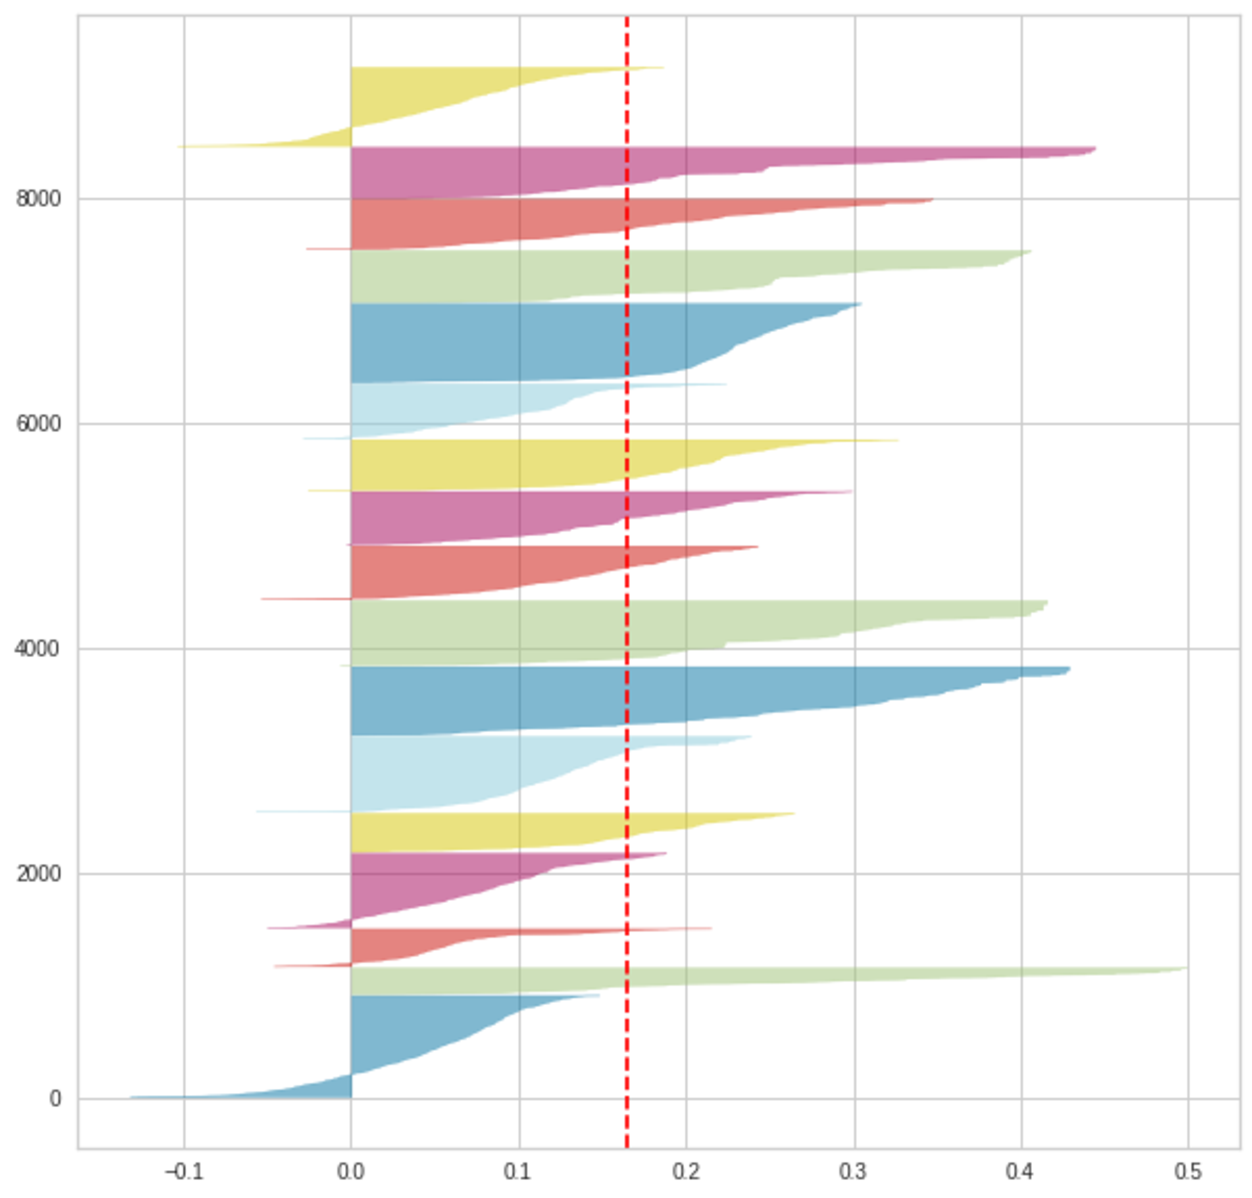
\includegraphics[width=\linewidth]{images/pre/silhouette_opc2_clustering.pdf}
\caption{Clusters consistency, through Silhouette scores.}
\label{fig:silohuette}
\end{figure}

\begin{figure}[ht!]
    \centering
    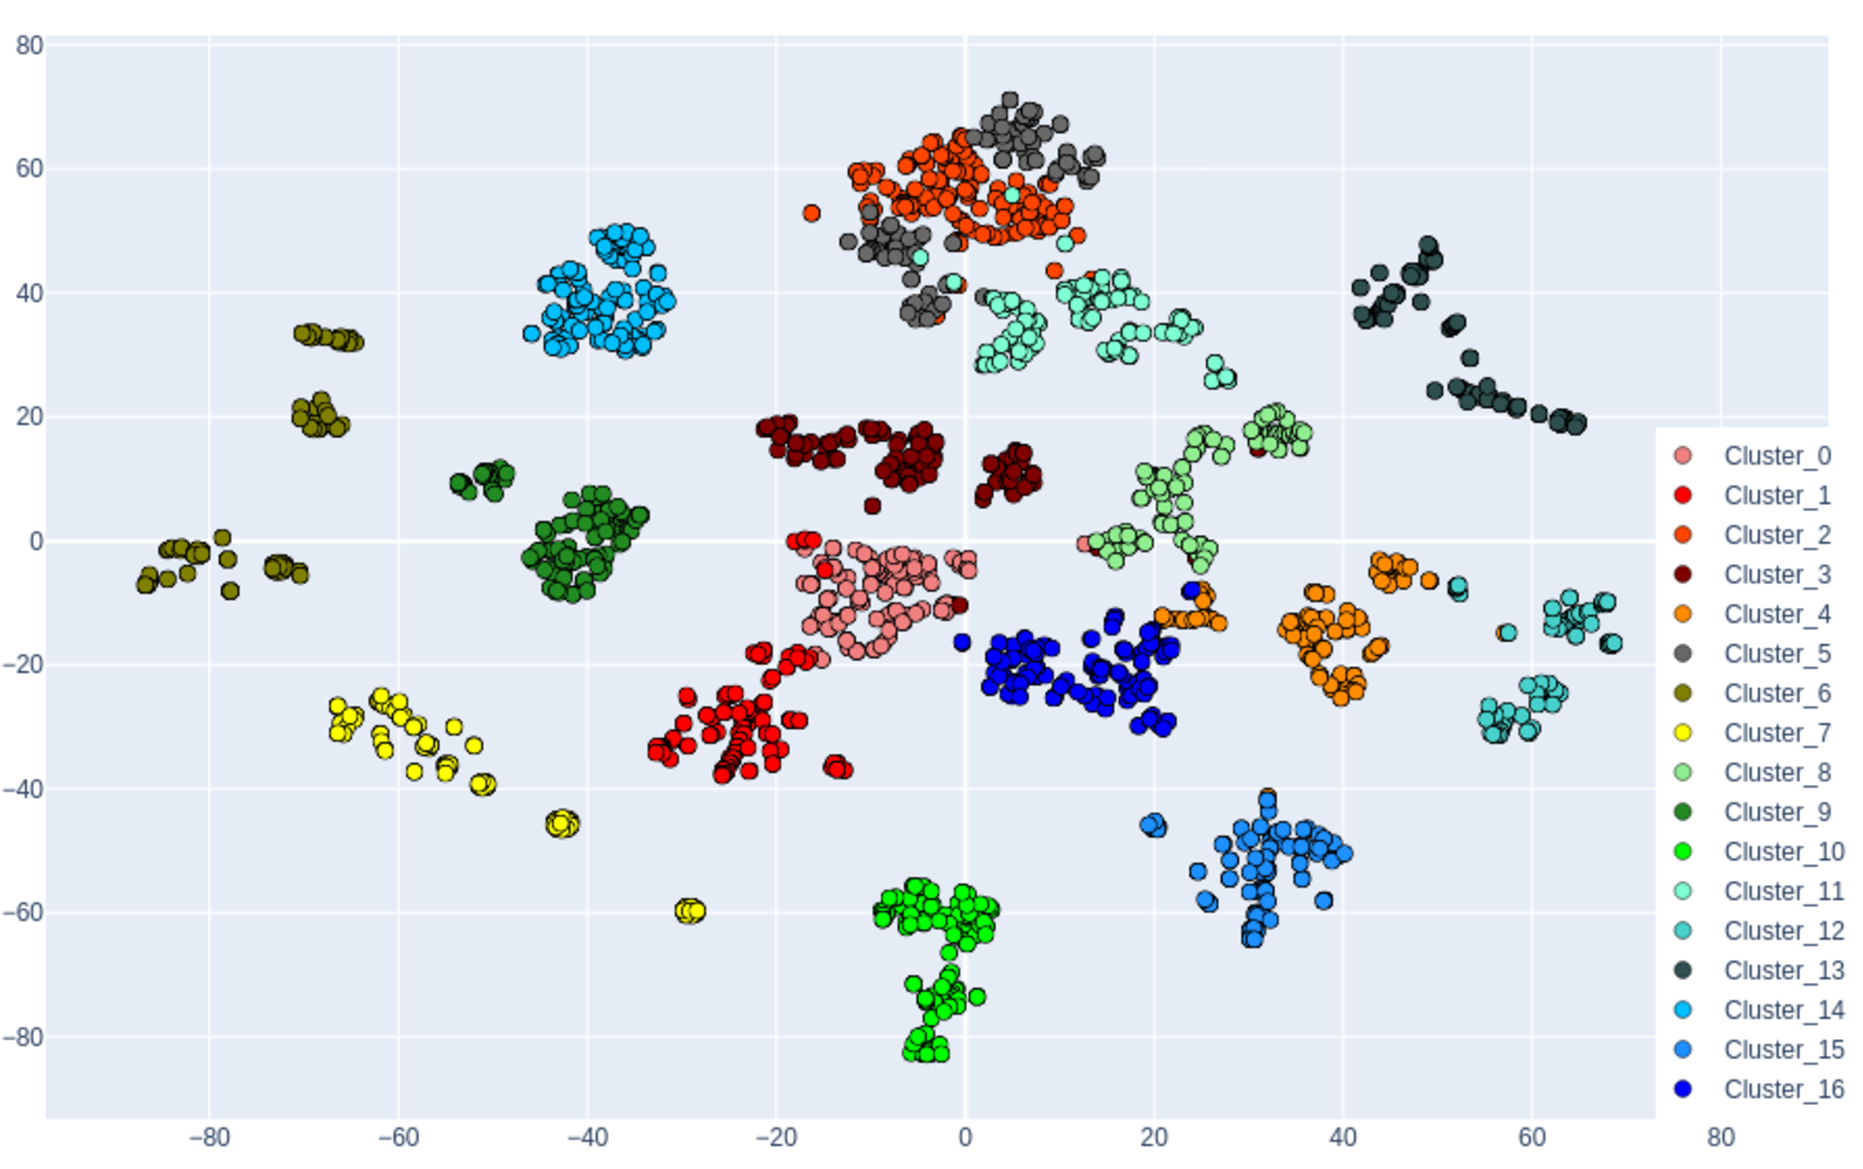
\includegraphics[width=\linewidth]{images/pre/plot2d_opc2_clustering.pdf}
\caption{Clusters distributions, displayed through T-SNE method.}
\label{fig:clustering2d}
\end{figure}


% Con respecto a los datos de entrada, esos resultaron de la concatenación de las listas de: \textbf{``lemas de pregunta + lemas de mejor respuesta''}; mientras que los embedding que alimentaron al algoritmo de Kmeans, se basaron en una matriz de ocurrencia con \textbf{1-gramas,...,10-gramas} como columnas de características. Una posterior reducción de dimensionalidad mediante umbral de varianza, descartó columnas de características con variaciones menores al \textbf{.001}, produjendo vectores finales de dimensionalidad \textbf{99}.
% Esta estrategia además, otorgó un \textbf{44.26\%} de precisión en las tuplas de control anotadas como pertenecientes a clusters similares, y un \textbf{99.33\%} para las anotadas como pertenecientes a clusters diferentes (Figura (\ref{fig:metrics})).
Regarding the input data, these resulted from the concatenation of the lists of: \textbf{`question lemmas + best answer lemmas'}; while the embeddings that fed the Kmeans algorithm were based on an occurrence matrix with \textbf{1-grams, ..., 10-grams} as feature columns, with a subsequent dimensionality reduction, using the technique of variance threshold, which discarded columns of characteristics with variations less than \textbf{.001}, producing final vectors with a dimensionality of \textbf{99}.
This strategy also gave a \textbf{44.26\%} precision in the control tuples annotated as belonging to similar clusters, and a \textbf{99.33\%} for those annotated as belonging to different clusters (Figure (\ref{fig:metrics})).

\begin{figure}[ht!]
    \centering
    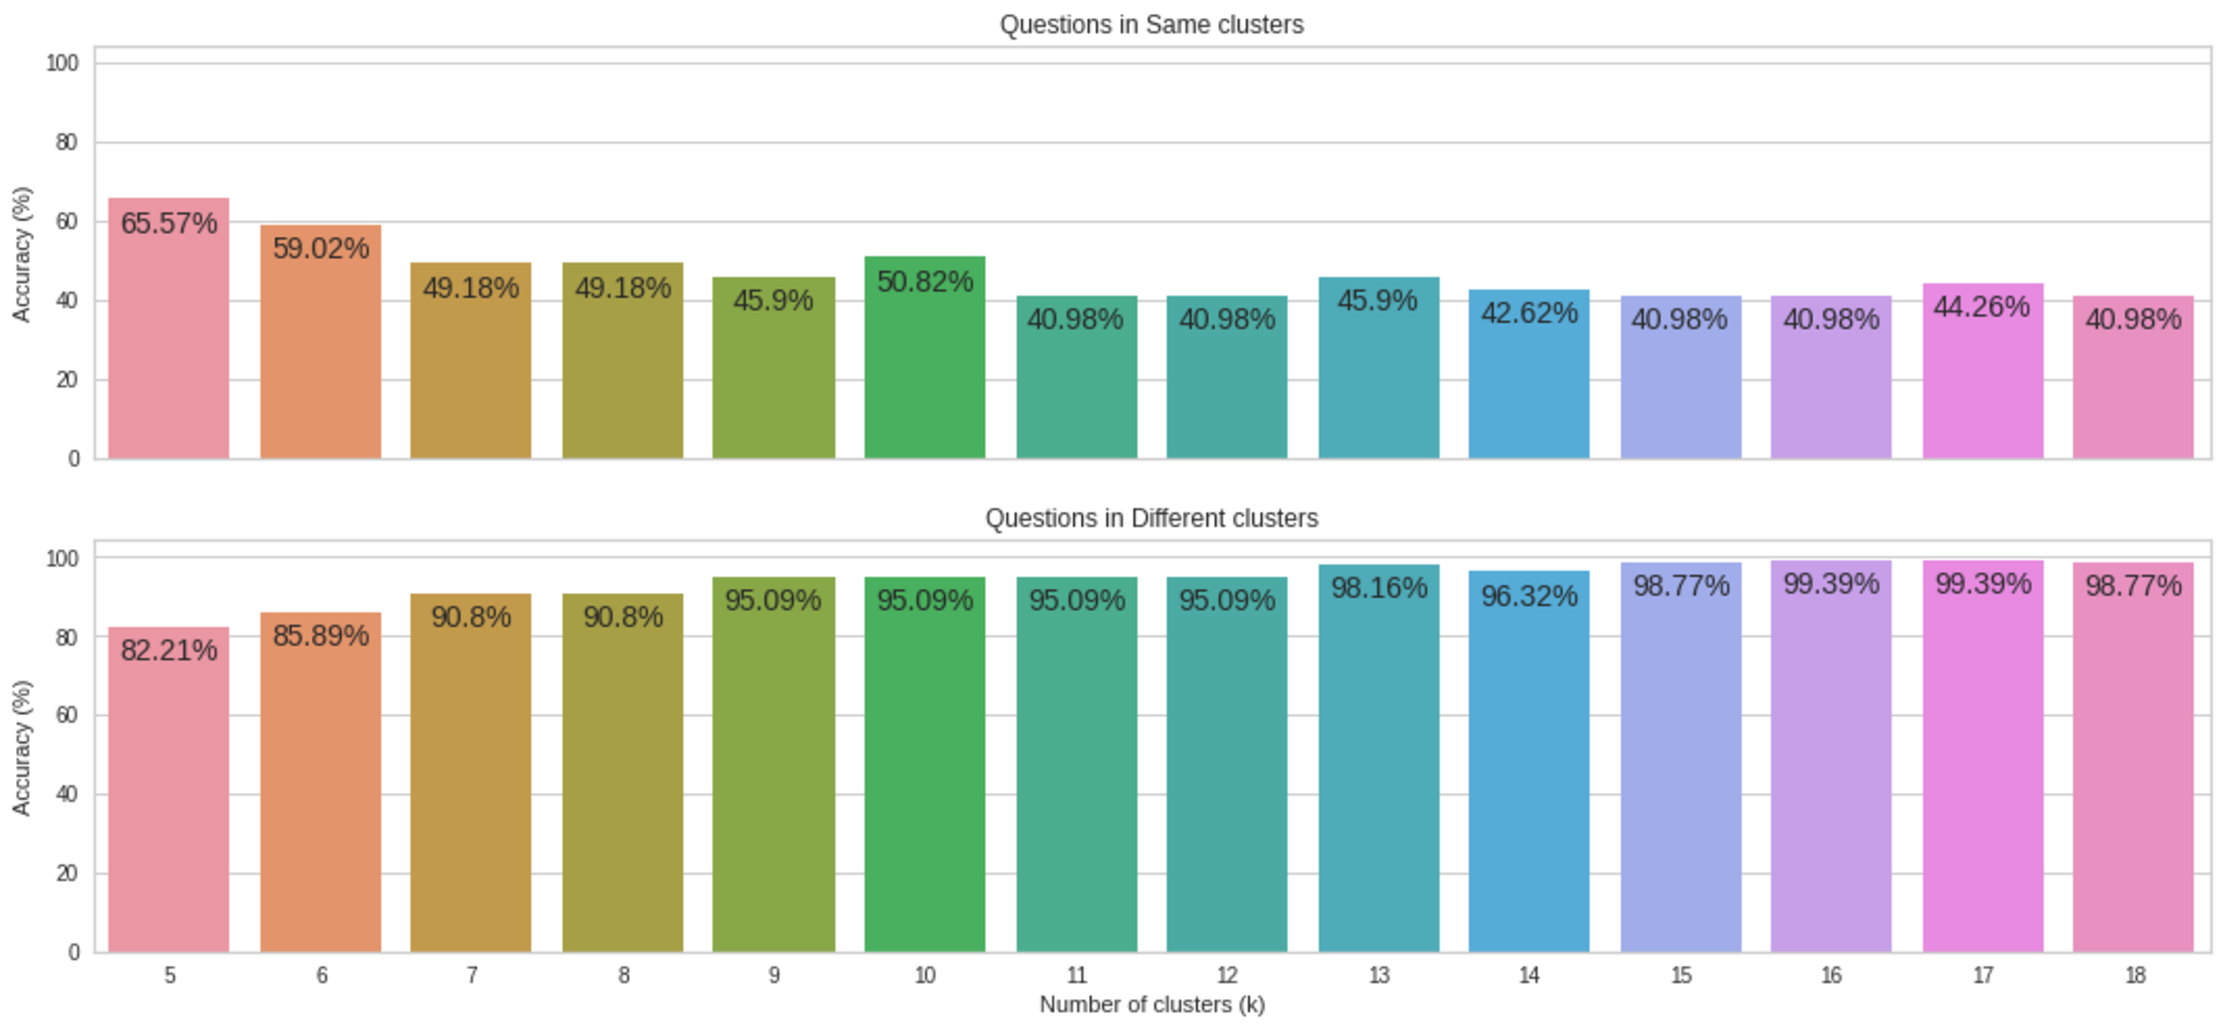
\includegraphics[width=\linewidth]{images/pre/metricts_opc2_clustering.pdf}
    \caption{Percentages of accuracy of the tuples considered to belong to the same clusters, and those considered to belong to different clusters, in relation to the results returned by the `KMeans' algorithm using a given k value.}
\label{fig:metrics}
\end{figure}

% En función de los resultados y experimentos realizados, se observó que las estrategias de clusterización basadas en embedding de tipo II fueron mucho mas ineficientes que las basadas en matrices de ocurrencia para algun rango de n-gramas. Tal observación, puede ser atribuida a la relativa poca cantidad de datos utilizados para la generación de los embedding, sumado a que los modelos utilizados no fueron pre-entrenados en conjuntos de datos de naturaleza conversacional.
% Por otro lado, los mejores rendimientos fueron alcanzados con datos de entrada construidos por concatenación de tokens de preguntas y respuestas lematizados. El aporte de respuesta con menos coincidencia generaron efectos negativos.
% Con respecto al la calidad de los clusteres, se notó que a medida que las preguntas se alejan de los centroides (ganan mayor distancia), se va perdiendo algo de consistencia. En linea general, se obtuvieron conjuntos de preguntas que comparten una mayor similitud morfológica que semántica, y están medianamente influenciados por sus respuestas. A pesar de ello, clusters como $0$, $1$, $5$ y $15$ resultaron de gran calidad y pureza, y combinaciones como $12$ y $13$, $16$ y $4$, entre otros, pudieron ser caracterizadas de manera muy precisa.
Based on the results and experiments carried out, it was observed that the clustering strategies based on type II embedding were much more inefficient than those based on occurrence matrices for some range of n-grams. Such observation can be attributed to the relative small amount of data used for the generation of the embedding, added to the fact that the models used were not pre-trained in datasets of a conversational nature.
On the other hand, the best performances were achieved using as input data, a concatenation of the question and answer lemma lists. It was also observed that the inclusion of answers with fewer coincidences produced a negative effect.
Regarding the quality of the clusters, it was noted that as the questions move away from the centroids (they gain greater distance), some consistency is lost. In general, sets of questions were obtained that share greater morphological than semantic similarity, and are moderately influenced by their answers. Despite this, clusters such as $0$, $1$, $5$ and $15$ were of great quality and purity, and combinations such as $12$ and $13$, $16$ and $4$, could be characterized very precisely.